\chapter{Evaluation}
\label{sec:evaluation}
\section{Comparison of different models}

\begin{equation}
	F1 = \frac{2 \times \text{TP}}{2 \times \text{TP} + \text{FN} + \text{FP}}
\end{equation}

The F1 score is a statistical measure used to evaluate the precision and recall of a model's predictions, essentially capturing the balance between the model's accuracy and its comprehensiveness in identifying relevant instances. Precision represents the accuracy of positive predictions, while recall measures the model's ability to identify all actual positive instances. The F1 score is the harmonic mean of precision and recall, thus ensuring that both metrics contribute equally to the final score, with a perfect F1 score being 1 and the worst being 0 \cite{chicco-2020}.

\begin{equation}
	\text{Weighted F1} = \sum_{i=1}^{N} w_i \times F1_i
\end{equation}

The weighted F1 score extends this concept by taking into account the class imbalance within a dataset. In scenarios where some classes are more prevalent than others, the weighted F1 score calculates a separate F1 score for each class, giving each score a weight proportional to the number of true instances for each class. This approach prevents the model's performance from being overly influenced by its effectiveness on the more common classes, instead emphasizing its overall performance across all classes. The weighted F1 score is particularly valuable in datasets with significant class imbalances, as it provides a more representative assessment of the model's predictive power \cite{leung-2022}.

\begin{table}[h]
	\centering
	\begin{tabular}{|l|l|l|l|l|}
		\hline
		Model            & weighted-F1 score \\ \hline
		CLIP             & \textbf{0.837}    \\
		Only designation & 0.779             \\
		Benchmark        & 0.814             \\
		\hline
	\end{tabular}
	\caption{Weighted-F1 scores}
	\label{tab:f1scores}
\end{table}

Table \ref{tab:f1scores} displays the range of weighted-F1 scores achieved by our model. These scores were obtained from a test set submitted to the challenge website, for which we did not have direct access to the true labels.

The CLIP model, which uses the designation and description field, as well as the images, got the best performance with an weighted F1 score of 0.837 (on the clean website test set). In contrast, the text-only model, which relies solely on product designations, achieved a weighted F1 score of 0.779 (on the clean website test set). While this model benefits from the informative nature of the product titles, it lacks the additional contex that images provide. The reduction in the weighted F1 score when compared to the full CLIP model underscores the value of incorporating visual features into the classification process.

The benchmark model, established by the challenge organizers, serves as a standard for comparison, achieving a weighted F1 score of 0.814 (on the clean website test set). While this model demonstrates a strong baseline performance, it falls short of the full CLIP model's capabilites.

It can be seen that integrating the images and the text data into one model gives better results than just using the text alone. It highlights the need for models that can effectively synthesize information from multiple sources, providing a more holistic view of the data at hand.

\section{Evaluation based on a confusion matrix}

A confusion matrix is a powerful tool for evaluating the performance of a classification model, providing a visual representation of the model's predictions compared against the actual labels. It not only reveals the instances of correct and incorrect predictions for each class but also uncovers the specific types of errors, such as which classes are being confused with others, enabling a nuanced analysis of the model's strengths and weaknesses \cite{susmaga-2004}.

We split our data into three parts: 80\% for training the model, 10\% for testing it, and another 10\% to validate how well it's doing. The confusion matrix we're looking at is based on this 10\% validation chunk.\\
The model provides an impressive 0.96\% f1 accuracy score on the validation data, we'll see in the future potential reasons why it did not worked as well on the clean website test set.\\

\begin{figure}[H]
	\centering
	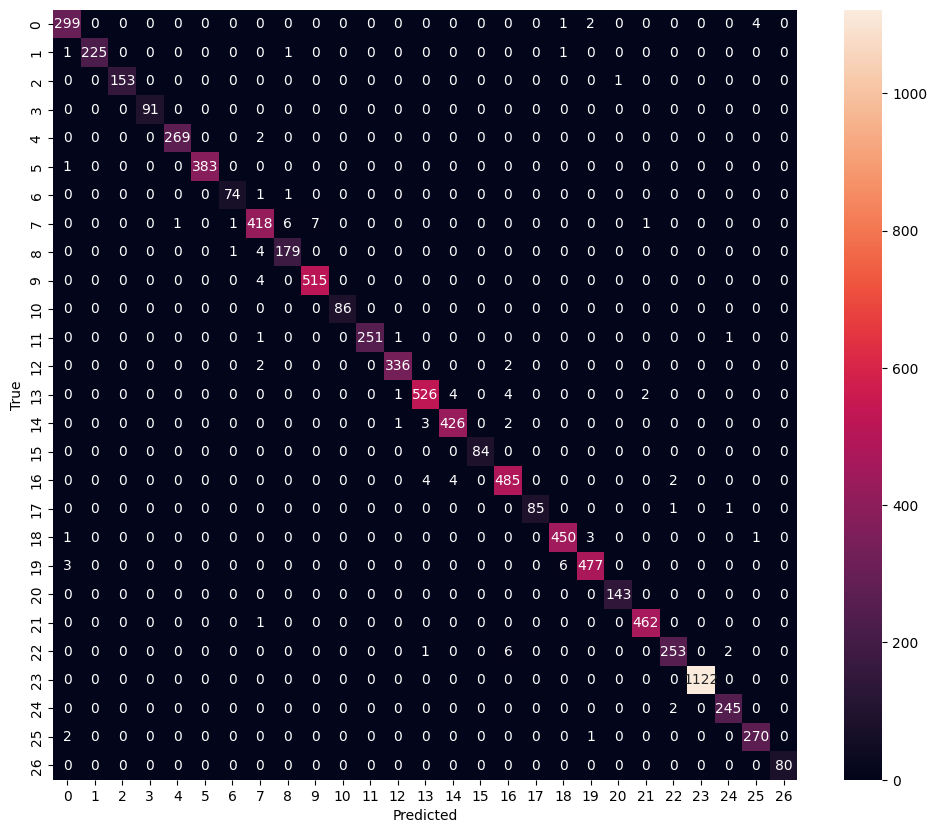
\includegraphics[width=1\textwidth]{confusion_matrix.png}
	\caption{Confusion matrix}
	\label{fig:confusionmatrix}
\end{figure}

The confusion matrix for our model gives us a clear picture of how well it's guessing the types of products. Most products are being placed in the right categories, which we can tell because there are lots of big numbers forming a line from the top left to the bottom right. This line shows where the model's guesses match the real answers.

While the model does a great job with many types of products, there are a few areas where it's not as accurate and could be better. But, there aren't too many mistakes overall, which is a good sign that our model isn't just memorizing the training data but actually learning from it.

This is confirmed by how well the model does on a completely new set of products it hasn't seen before, getting a score of 0.83. This means it's pretty good at applying what it's learned to new data.

Even though the confusion matrix might make us think the model has learned the training data too well, its good scores on both the validation data and the new test set from the challenge show that's not the case. It's not just repeating what it saw during training; it's making smart guesses on new products.

From the confusion matrix and the model's scores, it's clear that we've built a strong model that's good at figuring out what category different products belong to. It does well even with products it hasn't seen before, which proves our methods are working well.